\chapter{Standard integration methods}
% 16-11-2016 created


\label{ch:standardIntegrationMethods}
Propagation refers to the process of modelling/predicting the manner in which an object (for instance) will progress (in time) from a starting point, usually given an initial condition. Such an initial condition could be a constant force or another kind of perturbation. In orbital computations, numerical integration is often used to model this behaviour, because of the irregularities in the dynamic environment (many perturbations) and the absence of analytical solutions. The solution then provides an estimate of the trajectory and the state of the \ac{s/c}\citep{hofsteenge2013}. There are several different types of numerical integrators that all try to predict the \ac{s/c} behaviour in different ways. These types are described in \Cref{sec:differentIntegratorTypes}. In \Cref{sec:chosenMethodForComparison} the method is chosen that will be used in this research to compare the performance of the \ac{TSI} method with. \\
Numerical integration methods do have one major drawback compared to analytic methods, and that is the accuracy of the produced result. Numerical methods come close to the actual result but usually do not reach it. Therefore, there will always be a certain error associated with the answer. One of the most important errors is called the local (and total) truncation error, which is caused by the numerical inaccuracy of the method itself, and are usually the largest errors. A second error can be introduced by the round-off properties of the used computer, which then also depends on the number of evaluations required for each of the integration methods (more evaluations means more round-off errors). These round-off errors are due to the fact that computers can only accurately represent a number up until a certain number of decimal figures. According to \cite{milani1987} there are also specific errors that arise when integrating space-related problems. Instability errors can occur if the simulated system is chaotic or if the step-size is too large.\\
Another, non-method specific and not necessarily integration related, error source is the mistakes made in the physical model representing the problem in the simulation. Such errors can occur when forces and disturbances are not (properly) taken into account in the assumptions made to create the physical model.\\
Fortunately, many of the standard integration methods already contain functions that approximate these errors and then include those approximations to come up with a better solution, or try to minimize these errors by using multiple approximations. The focus of this chapter will thus be on the different integration methods and not the different methods of determining the different errors.

\section{Different integrator types}
\label{sec:differentIntegratorTypes}
A number of different numerical integration methods exist, however in this section they will be split based on how they work. In this case they have been split into single-step (\Cref{subsec:singleStep}) and multi-step methods (\Cref{subsec:multiStep}) based on \cite{noomen2013int}. The methods can also be split based on the used step-size; either a fixed step-size that does not change during the integration, or a variable step-size that changes per step (or sometimes even during the step). Finally, the methods can also be categorised by either being explicit or implicit. An explicit method uses the information provided at the start of the integration (the current state $\mathbf{x}_{i}$ and sometimes previous states) to determine the next state $\mathbf{x}_{i+1}$. Whereas an implicit method uses the same information to determine $\mathbf{x}_{i+1}$, but once this first solution is obtained, it uses this next state as an approximation of the solution and feeds it back into the method in order to determine a more accurate solution. This requires iteration. \\
The numerical approximation of the next state can be written as the current state plus the change during one time-step. This change is defined as the step-size $h$ times the increment function 
$\mathbf{\Phi}$ as shown by \Cref{eq:integration}, which changes depending on the method used. Here, $\mathbf{\eta}$ represents the total numerical approximation. 

\nomenclature[Ra5]{$\mathbf{x}_{i}$}{Current data point\nomunit{-}}
\nomenclature[Ra6]{$\mathbf{x}_{i+1}$}{Next data point\nomunit{-}}
\nomenclature[R4]{$h$}{(Current) step-size\nomunit{s}}
\nomenclature[G8]{$\Phi$}{Increment function\nomunit{-}}
\nomenclature[G3]{$\eta$}{Numerical approximation\nomunit{-}}


\begin{equation} \label{eq:integration}
\mathbf{x}(t_{0}+h)\approx\mathbf{x}_{0}+h\bm{\Phi}=\mathbf{\eta}(t_{0}+h)
\end{equation}

\nomenclature[Ra1]{$t_{0}$}{Initial time\nomunit{s}} 



\subsection{Single-step}
\label{subsec:singleStep}
Single-step methods solely use the information at the current point to determine the approximation of the next state. This means tht the information of the previous points is neglected and usually not saved \citep{noomen2013int}. Examples of the most simple explicit, fixed step-size, single-step methods are Euler, Mid-point and \ac{RK4} \citep{hofsteenge2013}. Euler uses the information at the current state to directly compute the estimate of the next state. Mid-point already incorporates an extra estimation where it first computes a point at half the step-size and then uses that information to approximate the next state, and \ac{RK4} takes 4 points into account and takes the weighted average of those to come up with a solution (the starting point, two mid-points and a final point). Many methods exists that are based on these simple methods, for instance the Mid-point method based high-order extrapolation (a.k.a. DIFEX2) (explicit) method \citep{deuflhard1994}.\\
Many more methods however are based on the \ac{RK4} principle such as Runge-Kutta-Nystr\"{o}m (RKN, with variations such as RKN7(6)9) (implicit) \citep{montenbruck1992,dormand1987}, \ac{RKN12} (implicit) \citep{montenbruck1992}  and \acf{RKF45} and \acf{RKF78} \citep{fehlberg1969,fehlberg1968}. These last two integrators are slightly different since they are still explicit, but use a variable step-size.


\subsection{Multi-step}
\label{subsec:multiStep}
Compared to the single-step method, the multi-step method does use the information of the previous points to estimate the next state. Usually reaching as far back as the previous three points such as the \ac{AB4} method \citep{noomen2013int}, this being the only difference between this method and the \ac{RK4} method. Extending this method creates the explicit \ac{AB6} method. An example of an implicit, fixed step-size, multi-step method is the Adams-Moulton method. It uses a polynomial to interpolate the function values in order to approximate the next state \citep{noomen2013int}. Explicit and implicit methods can also be combined to create so-called Predictor-Corrector methods. Here an initial guess is created by the explicit method, which is then fed into the implicit part in order to correct and improve the estimate. Examples of Predictor-Corrector methods are \ac{ABM4} and \ac{ABM12} \citep{noomen2013int,montenbruck1992}. \\
All previously mentioned multi-step methods use a fixed step-size. Variable step-size methods also exist, such as \ac{SG} (explicit) \citep{berry2004,meijaard1991} and \ac{SC14} (Predictor-Corrector) \citep{berry2004,ramos2005}.


\section{Chosen method for comparison}
\label{sec:chosenMethodForComparison}
In order to choose the method that will be used to compare the performance of \ac{TSI} to, it was important to understand which methods were readily available. If a method is already validated and available for use a lot of time can be saved. Therefore, an inquiry of available methods is made in \Cref{subsec:tudatMethods}. Another important criteria is that the performance of \ac{TSI} should be able to be compared to previous study cases. The easiest way of doing that is to see what methods other researchers used to compare \ac{TSI} to (see \Cref{subsec:methodsUsedInPreviousResearch}. Using the information from \Cref{subsec:tudatMethods,subsec:methodsUsedInPreviousResearch} a decision could be made on the final comparison method as is described in \Cref{subsec:chosenMethod}.

\subsection{Tudat methods}
\label{subsec:tudatMethods}
One of the software tools used in this thesis is \ac{Tudat} (see \Cref{subsec:tudat} for more information). It is a computational toolbox that already comes with a number of useful functions. It also contains a number of pre-programmed validated numerical integrators. A list of the available integration methods is provided in \Cref{tab:tudatIntegrators}.


\begin{table}[!ht]
\begin{center}
\caption{Available \ac{Tudat} integrators \citep{dirkx2016tudat}}
\label{tab:tudatIntegrators}
\begin{tabular}{|l|p{4cm}|p{8cm}|l|}
\hline 
\textbf{Method} & \textbf{Kind of method}		& \textbf{File} & \textbf{Ready for use} \\ \hline \hline
\ac{RK4} 	& explicit, fixed step-size, single-step & rungeKutta4Integrator.h & Yes  \\ \hline
\ac{RKF45} 	& explicit,  variable step-size, single-step & numericalIntegrator.h \& rungeKuttaVariableStepSizeIntegrator.h
\& rungeKuttaCoefficients.h/.cpp &  Yes \\ \hline
\acs{RKF56} 	& explicit, variable step-size, single-step & numericalIntegrator.h \& rungeKuttaVariableStepSizeIntegrator.h
\& rungeKuttaCoefficients.h/.cpp & No  \\ \hline
\ac{RKF78} &	explicit, variable step-size, single-step & numericalIntegrator.h \& rungeKuttaVariableStepSizeIntegrator.h
\& rungeKuttaCoefficients.h/.cpp &  Yes \\ \hline
\acs{DOPRIN87} 	& explicit, variable step-size, single-step & numericalIntegrator.h \& rungeKuttaVariableStepSizeIntegrator.h
\& rungeKuttaCoefficients.h/.cpp & Yes  \\ \hline
 	
 		
% 	&	&  &   \\ \hline
\end{tabular}
\end{center}
\end{table}

Most of these methods are very similar except \ac{RK4} which is a fixed step-size method, and \ac{DOPRIN87} which is actually a Runge-Kutta method similar to \ac{RKF} with an accuracy order 8(7) using the formulations as described by \cite{prince1981high} according to \cite{weeks2007comparison}. At the time of the research, the \ac{RKF56} method that was preprogrammed into \ac{Tudat} was unfortunately not available for use.

\subsection{Methods used in previous research}
\label{subsec:methodsUsedInPreviousResearch}
Out of the research done on integration methods for space missions, the most relevant is the research that was done on \ac{TSI}. The research performed by \cite{scott2008high} focused on orbital trajectories and used RKF8(9) and the researched performed by \cite{bergsma2016application} focussed on re-entry cases and used \ac{RKF56}. Unfortunately, RKF8(9) was not available through \ac{Tudat} and \ac{RKF56} was out of commission at the time of this thesis research. However, it is good to notice that both researchers used higher order RKF methods, which encourages the use of similar methods for this research and fortunately similar methods are available.

\subsection{Chosen method}
\label{subsec:chosenMethod}
Considering the available methods and the methods used in previous \ac{TSI} research it was determined that the \ac{RKF} methods and \ac{DOPRIN87} would be tested in the early phases of the verification process. In this case \ac{RK4} would serve as a back-up. During the verification of the standard integrator it was found that \ac{RKF78} showed the best performance when dealing with these ascent problems, which is why it was chosen as the integration method to which \ac{TSI} was later compared.


\section{Workings of \ac{RKF}}
\label{sec:rkf}
The principle behind \ac{RKF} is perhaps best explained by first looking at a simpler Runge-Kutta method such as \ac{RK4}. \cite{noomen2013int} provides a simple explanation of the workings of \ac{RK4} that have been adapted here. In this case, use is made of the general formulation for the numerical approximation as was shown in \Cref{eq:integration}. The increment function for \ac{RK4} is then presented by \Cref{eq:rk4_increment}. In this case four points are used to approximate the next state as visualised in \Cref{fig:rk4_noomen2013int}. 

\begin{equation} \label{eq:rk4_increment}
\Phi_{RK4}=\dfrac{1}{6}\left(k_{1}+2k_{2}+2k_{3}+k_{4}\right)
\end{equation}


\begin{figure}[!ht]
\centering
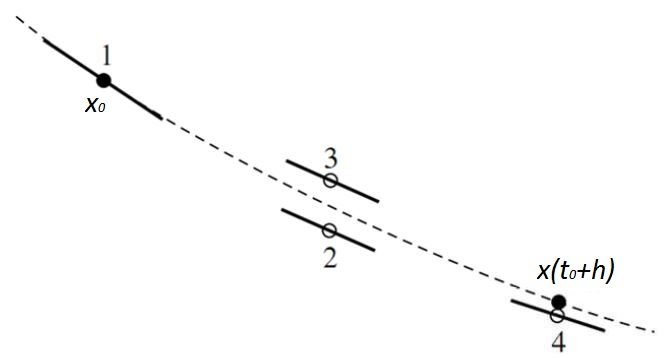
\includegraphics[width=0.3\textwidth]{figures/integrators/rk4_noomen2013int.jpg}
\caption{Principle of \ac{RK4} for a single parameter \cite{noomen2013int}.}
\label{fig:rk4_noomen2013int}
\end{figure}

Runge-Kutta works with the time-derivatives at those points. The derivative at the first point is called $k_{1}$, at the second point $k_{2}$ etcetera. These time derivatives are used both in the increment function but also in the process of determining the derivative of the next intermediate point as shown by \Cref{eq:k}.

\begin{equation} \label{eq:k}
\begin{split}
k_{1}&=f'\left(t_{0},\mathbf{x}_{0}\right)\\
k_{2}&=f'\left(t_{0}+h/2,\mathbf{x}_{0}+hk_{1}/2\right)\\
k_{3}&=f'\left(t_{0}+h/2,\mathbf{x}_{0}+hk_{2}/2\right)\\
k_{4}&=f'\left(t_{0}+h,\mathbf{x}_{0}+hk_{3}\right)\\
\end{split}
\end{equation}

\Cref{eq:rk4_increment,eq:k} can also be generalized as presented by \Cref{eq:generalRK}. In this case $b_{i}$ represents the different weights for each of the points with the corresponding step-size weights $c_{i}$, $n$ is the order and $a_{i,j}$ are the coefficients of the previous time-derivatives.

\begin{equation} \label{eq:generalRK}
\begin{split}
\Phi_{RK} &= \displaystyle \sum^{n}_{i=1}b_{i}k_{i} \\
\text{with}\quad k_{i} &= f'\left(t+c_{n}h,y+h\displaystyle \sum^{n-1}_{j=1}a_{i,j}k_{j} \right) \\
\end{split}
\end{equation}


This general formulation can now also be used to compute the higher order Runge-Kutta approximations given that $a_{i,j}$, $b_{i}$ and $c_{i}$ are provided. These sets of numbers can be found in various literature, and different people have come up with different sets. Fehlberg was one of these people. In order to get a more accurate solution he decided to use two different methods. In the case of this research, \ac{RKF78} was used, which means that a 7$^{th}$ order and 8$^{th}$ order solution can be computed using \Cref{eq:generalRK}. The 7$^{th}$ order solution is then used as the method solution and the difference between the 8$^{th}$ and the 7$^{th}$ order solution results in an error estimate which can be used to determine the next step-size. This step-size is thus computed such as to minimize this error estimate. This means that the only difference between \ac{RKF78} and \ac{RKF45} (for instance) is the coefficient set (a, b and c's). 









